\documentclass[12pt]{article}

\usepackage{blindtext}
%Image-related packages
\usepackage{graphicx}
\usepackage{subcaption}
\usepackage[export]{adjustbox}
\usepackage{wrapfig}
\usepackage{subfigure}
\graphicspath{ {./images/} }

%------------------------------

\usepackage{tabularx} % extra features for tabular environment
\usepackage{siunitx}
\usepackage{enumerate}
\usepackage{amsmath}  % improve math presentation
\usepackage{graphicx} % takes care of graphic including machinery
\usepackage{cite} % takes care of citations
\usepackage[margin=1in,letterpaper]{geometry} 
\usepackage{textcomp}
\usepackage{pgfplots}
\pgfplotsset{width=5cm, compat=1.9}

\usepackage[final]{hyperref} % adds hyper links inside the generated pdf file
\usepackage{framed}
\hypersetup{
	colorlinks=true,       % false: boxed links; true: colored links
	linkcolor=blue,        % color of internal links
	citecolor=blue,        % color of links to bibliography
	filecolor=magenta,     % color of file links
	urlcolor=blue         
}
\usepackage{listings}
\usepackage{xcolor}      %代码着色宏包
\usepackage{CJK}         %显示中文宏包

\usepgfplotslibrary{external}
\tikzexternalize

\lstset{
    basicstyle=\tt,
    %行号
    numbers=left,
    rulesepcolor=\color{red!20!green!20!blue!20},
    escapeinside=``,
    xleftmargin=-2em,xrightmargin=-2em, aboveskip=1em,
    %背景框
    framexleftmargin=0 mm,
    frame=shadowbox,
    %背景色
    backgroundcolor=\color[RGB]{245,245,244},
    %样式
    keywordstyle=\color{blue}\bfseries,
    identifierstyle=\bf,
    numberstyle=\color[RGB]{0,192,192},
    commentstyle=\it\color[RGB]{96,96,96},
    stringstyle=\rmfamily\slshape\color[RGB]{128,0,0},
    %显示空格
    showstringspaces=false
}
%++++++++++++++++++++++++++++++++++++++++

\begin{document}
%%%% Header Information %%%%
\include{header}

%%%% Document Information %%%%
\title{\fontsize{25}{15}\selectfont Final Project: On-Chip Neural Chess Analyzer}
\author{Haihan Wu, MIT ID:941455864}
\date{December \(9^{th}\) 2022}
%%%%%%% End Document Header %%%%%%%
\maketitle

\section*{Part I: Tiny-TPU background}
\subsection*{1. Deep Neural Networks and Accelerators}
Deep neural networks (DNNs) are utilized for many artificial intelligence applications because it performs more accurate results on different AI tasks, however, the computation complexity is high. The main DNN computation consists of convolution, matrix multiplication, max-pooling and non-linearity. To compute the output of DNNs faster, the hardware accelerators are designed to process parallel data.
The core operation for accelerators is multiply-and-accumulate (MAC) operation, which is performed by the processing elements (PE). 

\subsection*{2. Systolic Array}
A systolic array can efficiently implement matrix multiplication in hardware. Google Tensor Processing Unit(TPU) uses a systolic array architecture. A systolic array consists of processing elements (PEs), and the simplest processing element is divided into weight-stationary(figure 1.(a)) and output-stationary(figure 1.(b)): \\
\begin{figure}[h]
\begin{center}
\begin{subfigure}{0.3\textwidth}
\begin{center}
\includegraphics[width=0.9\linewidth, height=4cm]{WS.png} 
\caption{Weight stationary PE}
\label{fig:subim1}
\end{center}
\end{subfigure}
\begin{subfigure}{0.3\textwidth}
\begin{center}
\includegraphics[width=0.9\linewidth, height=4cm]{OS.png}
\caption{Output stationary PE}
\label{fig:subim2}
\end{center}
\end{subfigure}
\end{center}
\caption{Two typical types of processing elements}
\label{fig:image2}
\end{figure}
\\
A systolic array composed of weight-stationary PEs needs to store the weight matrix in each processing element in advance. The processing element will add the partial sum transmitted from the previous processing element to the product of the input and weight of this element, and then transfer the accumulated sum to the next processing element. Therefore, the weight-stationary systolic array will output the result matrix in the form of pulse data. The Google first generation of TPU utilized this PE. On the contrast, the output-stationary processing element accepts input and weight, and continues to accumulate the product of different input and weight, and the result is stored in the processing element.\\
\\
In terms of convolution, several ways are mentioned in Professor Sze's survey paper about DNN accelerator designs$^{[1]}$. One way is to flatten the weight kernel and transform the two-dimensional input matrix, and then multiply the two transformed matrices. However, it's less efficient especially when ifmap is very large. Another method is to use fast Fourier transform (as shown in the figure 2(b)).\\
\begin{figure}[h]
\begin{center}
\begin{subfigure}{0.4\textwidth}
\begin{center}
\includegraphics[width=1\linewidth, height=8cm]{conv_app_1.png} 
\caption{Approach 1: matrix transform}
\label{fig:subim1}
\end{center}
\end{subfigure}
\begin{subfigure}{0.4\textwidth}
\begin{center}
\includegraphics[width=1\linewidth, height=5cm]{conv_app_2.png}
\caption{Approach 2: fft()}
\label{fig:subim2}
\end{center}
\end{subfigure}
\end{center}
\caption{Two convolution method}
\label{fig:image2}
\end{figure}
\\
In this project, tiny-TPU uses a similar approach to fast Fourier transform: first, the weight kernel is placed in the weight-stationary pulse array, and then the number of rows of the same height as the weight kernel are continuously extracted from the input and transformed into systolic data, which is sent to the pulse array; subsequently, the elements of all rows of the output array are added, and after filtering, a row of output is obtained. Repeating the above operation can obtain the result of the convolution. 

\subsection*{3. Tiny-TPU Working Principles}
Figure 3 illustrates matrix multiplication and convolution.\\
\begin{figure}[h]
\begin{center}
\begin{subfigure}{0.4\textwidth}
\begin{center}
\includegraphics[width=1\linewidth, height=6cm]{tpu_conv.png} 
\caption{Tiny-TPU convolution}
\label{fig:subim1}
\end{center}
\end{subfigure}
\begin{subfigure}{0.4\textwidth}
\begin{center}
\includegraphics[width=1\linewidth, height=6cm]{tpu_mul_correct.png}
\caption{Tiny-TPU matrix multiplication}
\label{fig:subim2}
\end{center}
\end{subfigure}
\end{center}
\caption{Tiny-TPU Operation}
\label{fig:image2}
\end{figure}
\\ 
The input is a systolic data of 3 rows. The weights are pre-stored in systolic array and output are at the bottom. All the output elements are represented by the column vector inner products as $a_i$·$w_j$. The outputs are valid inside the red rectangles. For multiplication, all of the systolic output are valid and will be further processed into a matrix. If we want the result of matrix A and W, one thing should be noticed that each output element is inner product of row of A and column of W. So the input matrix should be transposed and then converted to systolic data form.\\
\begin{figure}[h]
\begin{center}
\begin{subfigure}{0.4\textwidth}
\begin{center}
\includegraphics[width=1\linewidth, height=6cm]{tpu_mul_wrong.png} 
\caption{Input without transpose}
\label{fig:subim1}
\end{center}
\end{subfigure}
\begin{subfigure}{0.4\textwidth}
\begin{center}
\includegraphics[width=1\linewidth, height=6cm]{tpu_mul_correct.png}
\caption{input with transposed}
\label{fig:subim2}
\end{center}
\end{subfigure}
\end{center}
\caption{Tiny-TPU matrix multiplication}
\label{fig:image2}
\end{figure}
\\ 
As to Convolution, if weight matrix is 3-by-3, then the buffer sends 3 rows of the input in systolic data form each time. On figure 3(a), one interesting thing is that the weight matrix stored is horizontally flipped. The reason is that the valid output of convolution is ($a_1$$w_1$+$a_2$$w_2$+$a_3$$w_3$), ($a_2$$w_1$+$a_3$$w_2$+$a_4$$w_3$) ... ($a_{n-2}$$w_1$+$a_{n-1}$$w_2$+$a_n$$w_3$), and the output on each column is the inner products of the input column and the corresponding weight column, e.g., the outputs of the first column are dot-products of input columns and \textbf{w$_1$}. To get the output, the output elements of the same row are summed. \\
\\
The tiny TPU design below will follow this principle and realize DNN computation.

\section*{Part II: Tiny-TPU Architecture}
\subsection*{1. Tiny-TPU architecture}
The whole block diagram for tiny-TPU is given below:\\
\begin{figure}[h]
\begin{center}
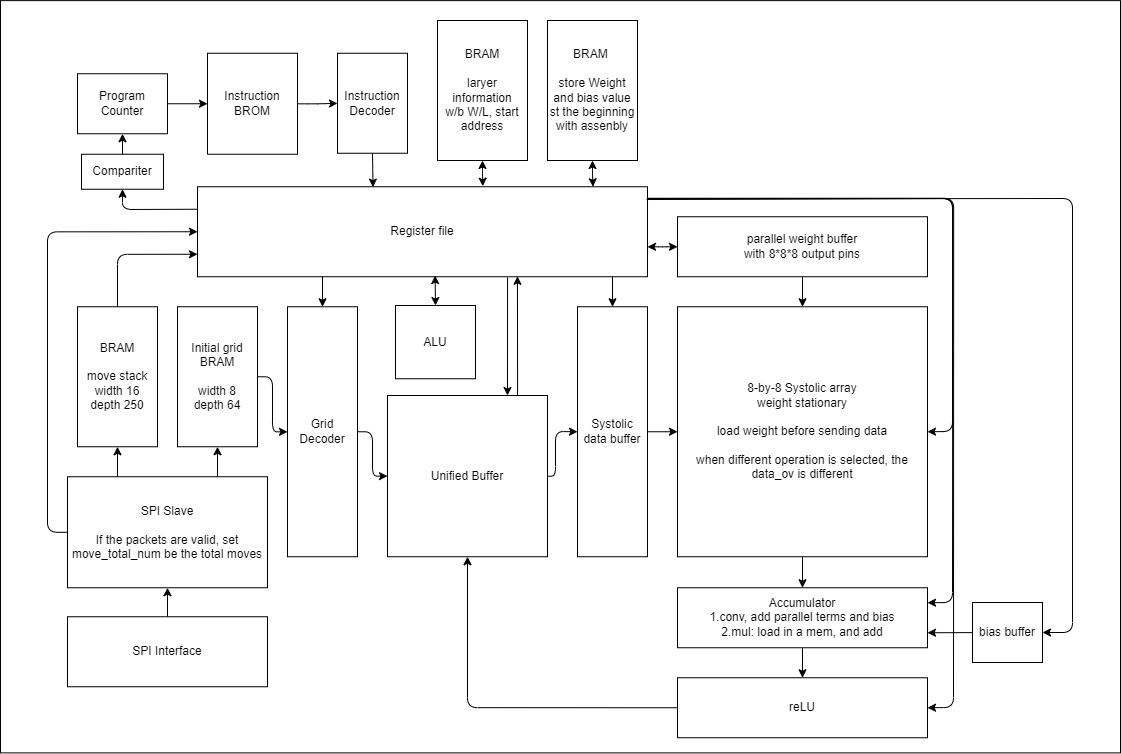
\includegraphics[width=1\textwidth]{TPU_v1.png}
\caption{Tiny TPU Block Diagram}
\label{fig:image2}
\end{center}
\end{figure}
\\
Instructions are stored in instruction block ROM, layer information, weights and biases are stored in the main memory. When the TPU receives packet from the move generator through SPI, it will check the packet first. If the received data complies with the encoding, then the TPU stores the initial grid in distributive ram and all the possible moves in move stack. After that, the nonzero total move number is loaded in the register file module, which activates the DNN computation program. The register file module has 3 groups of 64 registers: the first group load encoded layer information from main memory and further decode it into detailed layer static

\subsection*{2. Computation Architecture}
\begin{figure}[h]
\begin{center}
\includegraphics[width=1\textwidth]{Comp_arch.png}
\caption{TPU single-cycle computation architecture}
\label{fig:image2}
\end{center}
\end{figure}

\subsection*{3. C and Assemble program}

\subsection*{4. Special instrucions}

     
\section*{Part III: Design Verification}

\section*{Part IV: Assembly Program}

\section*{Part V: Reference}
[1] V. Sze, Y. -H. Chen, T. -J. Yang and J. S. Emer, "Efficient Processing of Deep Neural Networks: A Tutorial and Survey," in Proceedings of the IEEE, vol. 105, no. 12, pp. 2295-2329, Dec. 2017, doi: 10.1109/JPROC.2017.2761740.

\end{document}